\normaltrue \difficilefalse \tdifficilefalse
\correctionfalse

%\UPSTIidClasse{11} % 11 sup, 12 spé
%\newcommand{\UPSTIidClasse}{12}

\exer{EPAS $\star$ \label{B2:10:64}}
\setcounter{question}{0}\UPSTIcompetence[2]{B2-10}
\index{Compétence B2-10}
\index{EPAS}
\ifcorrection
\else
\marginnote{\textbf{Pas de corrigé pour cet exercice.}}
\fi



\ifprof
\else
Dans une première approche, on modélise le parc échelle d'un camion de pompier par un assemblage de trois plaques
rectangulaires homogènes d’épaisseur négligeable, de longueur $L$ et de largeur $h$. Chaque plaque a une masse notée $m$.


\begin{figure}[H]
\centering
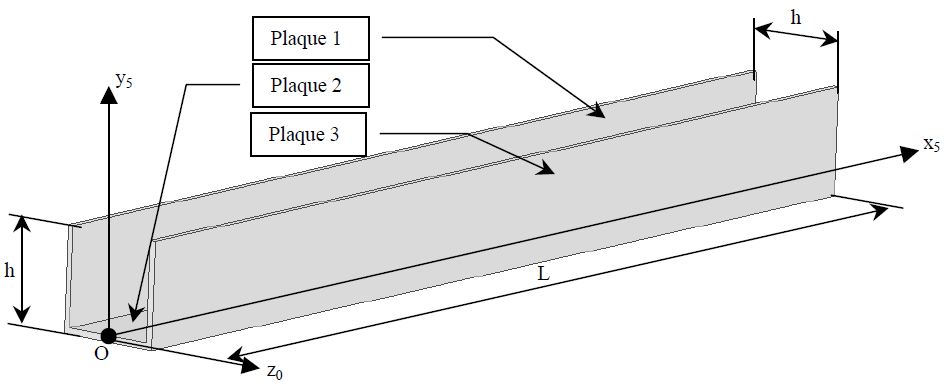
\includegraphics[width=\linewidth]{64_01}
\end{figure}
\fi

\question{Montrez que le vecteur position $\vect{OG}$ du centre de gravité $G$ du parc échelle est tel que $\vect{OG}=\dfrac{L}{2}\vect{x_5}+\dfrac{h}{3}\vect{y_5}$.}
\ifprof
\else
\fi



\ifprof
\else
\begin{flushright}
\footnotesize{Corrigé voir \ref{B2:10:64}.}
\end{flushright}%
\fi